\section{Diagrama Entidad-Relaci\'on (DER)}

\subsection{Diagrama}
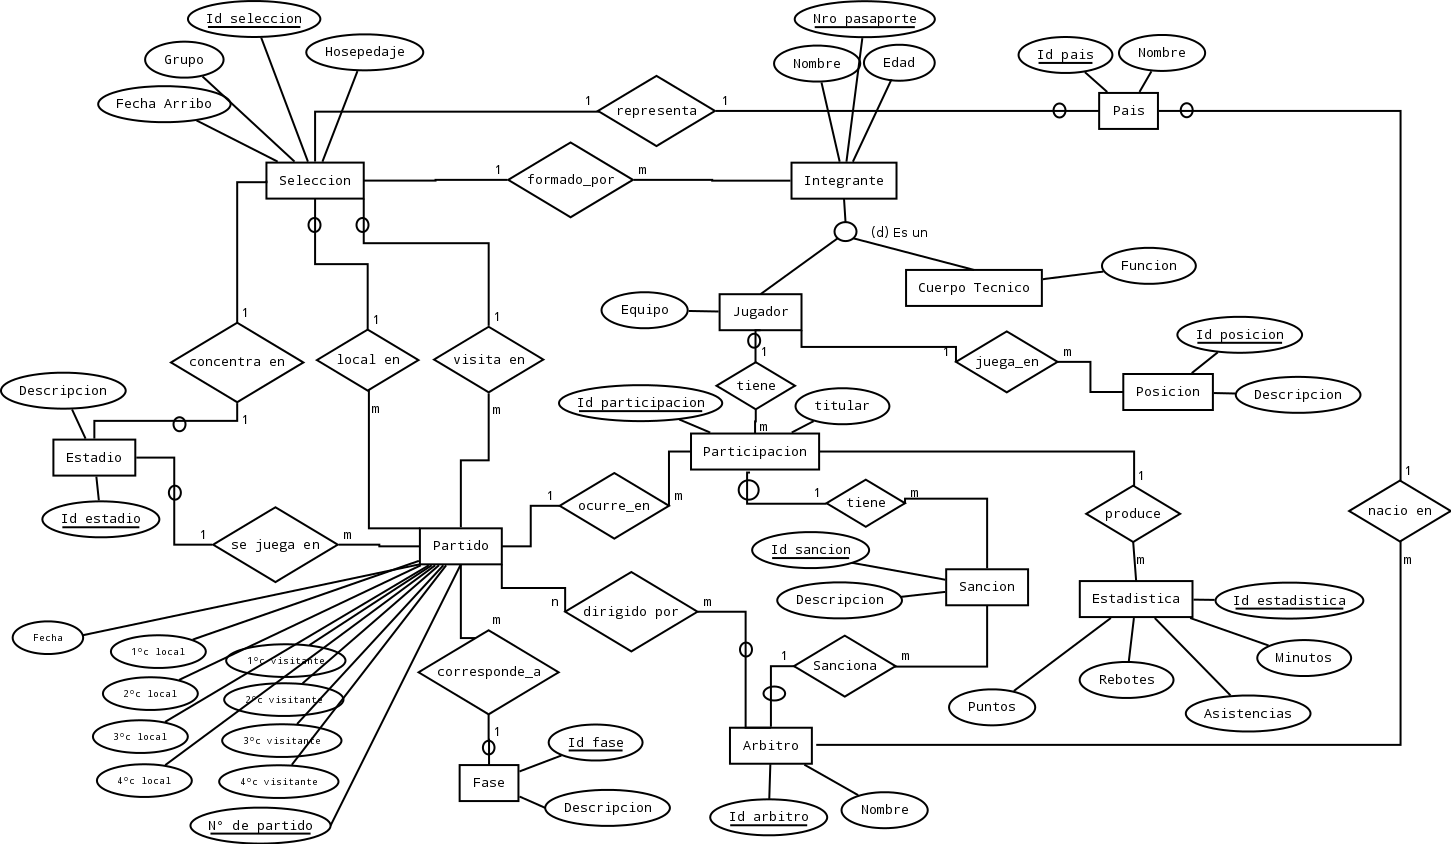
\includegraphics[scale=0.4, angle=90]{imgs/Der.png}


\newpage

\subsection{Decisiones de Dise\~no}


Para comenzar con el trabajo lo primero que hicimos fue tratar de identificar en el texto todo aquello que consderabamos que podia llegar a ser una entidad, para ellos seleccionamos del texto las palabras claves tales como, Jugador, Estadistica, Partido, Seleccion etc.
Luego detectamos que hab\'ia atributos tales, como pais y estadio que se usaban de manera repetidas, por lo que decidimos pasar a estas tambien en forma de Entidades.
Una vez con las entidades definidas nos propusimos llevar adelante la correcta diagramación de las interelaciones
Si bien no encontramos dificultades para poder relacionar las entidades, nos encontramos con una traba para poder relacionar al partido, con las estad\'isticas y con los jugadores
A primera instancia tratamos de trabajar con las estad\'isticas de forma que se generaban de manera agregada de la relaci\'on entre partido y jugador, sin embargo desistimos de esta opci\'on ya que no es posible que no exista estad\'istica alguna de un jugador que jugo un partido, por lo que no es necesario este tipo de relaci\'on.
Intentamos hacer una relaci\'on de grado 3 sin embargo tampoco creimos que era la manera correcta porque nos obligaba a inicializar una planilla de estadistica sobre todos los jugadores con valores en 0 y esto no es correcto, sino que las estad\'isticas se realizan sobre los jugadores que juegan. 
Finalmente decidimos implementar una entidad participaci\'on, encargada de administrar las estadisticas, si un jugador fue titular o no en ese partido y si tuvo o no sanciones.
A medida que ibamos diagramando nos encontramos con la necesidad de tomar decisiones para que el diagrama creado sea leído de manera correcta.

\begin{itemize}
\item Decidimos implementar la relaci\'on de partido con selecci\'on con dos relaciones distintas, la cual uno pertenece a una selecci\'on que hace el modo de Local y la otra de Visitante, es importante indicar que se debe restringir que esta selecci\'on no sea la misma, ya que esto es imposible en la realidad.
\item Por partido solo puede haber una cantidad de 12 jugadores correspondientes a cada equipo, es decir que si bien la relaci\'on es en base a $m$ este se limita a solamente 12
\item Se debe restringir que la cantidad de titulares de un partido sea igual a 5 tal como lo indica el trabajo para ello creamos un trigger en el cual si se intenta cargar un jugador como titular y ya se alcanzo la cantidad maxima, esa inserción falla.
\item Asumimos que la posici\'on de un jugador es propia del mismo e independientemente del partido, tal como es en la realidad de las estadisticas del basquet.
\item Permitimos que haya mas de un arbitro por partido, ya que entendemos que el enunciado asi lo pide refiriendose constantemente al terma arbitraje como plural
\item Si bien el partido tiene muchos \'arbitros, una sanci\'on puede ser aplicada por un solo \'arbitro.
\item Decidimos no colocar un campo de resultado final dentro de la tabla partido ya que este campo se puede deducir de la suma de los cuartos correspondientes a cada selecci\'on.
\item Si bien el trabajo solicita que se almacenen solo las estad\'isticas de los mejores jugadores, tambien pide como item emitir un reporte de las mismas sobre todos los que jugaron, por lo que no solo almacenamos informacion de los mejores sino que la haremos sobre todos los jugadores con partidos en su haber.
\end{itemize}


